\documentclass[UTF8]{ctexart}
% 加载必要宏包(补充表格美化、超链接功能)
\usepackage{graphicx}   % 插入图片
\usepackage{amsmath}    % 数学公式
\usepackage{siunitx}    % 单位格式
\usepackage{caption}    % 图表标题
\usepackage{booktabs}   % 美观表格(三线表)
\usepackage{hyperref}   % 可点击超链接
\usepackage{enumitem}   % 列表格式控制(避免序号错乱)



% 文档元信息(优化标题表述,更贴合内容)
\title{耳机(含蓝牙耳机)的工作原理与技术解析}
\author{薛中州}
\date{\today}

% 超链接格式设置(避免中文乱码,统一蓝色样式)
\hypersetup{
    colorlinks=true,
    linkcolor=blue,
    urlcolor=blue,
    citecolor=blue
}

\begin{document}
\maketitle
\pagestyle{plain}  % 统一页脚格式(避免章节页脚混乱)

% 目录与图表目录(调整顺序,先目录后图表目录,符合中文文档习惯)
\tableofcontents  % 新增文档目录,方便跳转
\listoftables     % 表格目录
\listoffigures    % 图片目录
\clearpage        % 分页,避免目录与正文混杂

% 摘要(补充标题,明确范畴,修正逻辑)
\begin{abstract}
\textbf{摘要:} 耳机是现代生活中不可或缺的音频设备,其中蓝牙耳机凭借无线便携特性,在青少年及职场人群中广泛普及。本文结合声学、电磁学基础知识,先明确耳机的通用分类维度,再分别解析「通用耳机的核心结构与声音还原原理」及「蓝牙耳机的特殊组件与无线连接原理」,最后给出耳机使用与维护建议,旨在帮助读者系统理解耳机技术特性,为选购与使用提供参考。
\end{abstract}
\clearpage

% 第一章:耳机的分类(新增章节,先明确分类逻辑,避免后续范畴混淆)
\section{耳机的分类}
耳机分类维度多样,核心可按「佩戴方式」与「连接方式」划分为两大类,不同类型的结构与适用场景差异显著(见表\ref{tab:earphone_classification})。

\begin{table}[htbp]  % 优化表格位置参数(h:当前页,t:顶部,b:底部,p:单独页)
    \centering
    \caption{耳机的核心分类(按佩戴方式与连接方式)}
    \label{tab:earphone_classification}
    \begin{tabular}{c c c c}  % 四列布局,明确分类维度
        \toprule  % 顶部粗线(三线表样式)
        \textbf{分类维度} & \textbf{具体类型} & \textbf{佩戴/连接特点} & \textbf{核心适用场景} \\
        \midrule  % 中间细线
        \multirow{2}{*}{佩戴方式} & 头戴式耳机 & 耳罩全覆盖外耳,头带固定 & 居家听感、专业音频监听(长时间佩戴舒适) \\
                                  & 入耳式耳机 & 耳塞插入耳道,轻量化设计 & 运动、通勤(便携且被动隔音好) \\
        \midrule
        \multirow{2}{*}{连接方式} & 有线耳机   & 依赖3.5mm/Type-C线缆传输信号 & 专业录音、HiFi听音(信号传输稳定,无延迟) \\
                                  & 蓝牙耳机   & 通过蓝牙协议无线传输信号   & 日常通勤、运动(摆脱线缆束缚,便携性强) \\
        \bottomrule  % 底部粗线
    \end{tabular}
    \caption*{注:「头戴式/入耳式」可与「有线/蓝牙」交叉组合(如头戴式蓝牙耳机、入耳式有线耳机),表中为核心分类维度的典型组合。}
\end{table}

% 第二章:耳机的核心结构(区分「通用组件」与「蓝牙耳机特殊组件」,修正范畴混淆)
\section{耳机的核心结构}
耳机结构需按「通用组件」与「蓝牙耳机特殊组件」区分:前者是所有耳机的基础,后者仅为蓝牙耳机特有(见图\ref{fig:earphone_structure})。

\begin{enumerate}[label={\arabic*.}, itemsep=6pt]  % 控制列表间距,提升可读性
    \item \textbf{通用核心组件(所有耳机必备)}
    \begin{enumerate}[label={\arabic{enumi}-\arabic*.}, itemsep=3pt]  % 二级列表,明确层级
        \item \textbf{扬声器单元}:将电信号转换为声波的核心部件,主流类型有三类:
              - 动圈式:成本低、频响宽,适合大众消费级耳机;
              - 动铁式:解析力强、体积小,多用于高端入耳式耳机;
              - 静电式:失真低、音质细腻,常见于高端HiFi耳机。
        \item \textbf{耳罩/耳塞}:头戴式用耳罩(多为海绵/皮质,提升舒适度),入耳式用耳塞(硅胶/记忆棉材质,隔绝外界噪音)。
        \item \textbf{连接与固定部件}:头戴式靠「头带」固定,入耳式/有线头戴式靠「音频线缆」传输信号(蓝牙耳机无此线缆)。
    \end{enumerate}

    \item \textbf{蓝牙耳机特殊组件(仅蓝牙耳机具备)}
    \begin{enumerate}[label={\arabic{enumi}-\arabic*.}, itemsep=3pt]
        \item \textbf{蓝牙模块}:含蓝牙芯片与天线,支持SBC、AAC、aptX等主流音频协议(其中AAC、aptX音质优于基础SBC协议),实现与手机/电脑的无线连接。
        \item \textbf{电池单元}:多为锂离子电池(容量通常为50-500mAh),为蓝牙模块、内置放大器供电,单次续航普遍为4-20小时。
        \item \textbf{控制芯片}:负责蓝牙信号解码、音量调节、通话降噪等功能,部分高端机型还集成主动降噪(ANC)模块。
    \end{enumerate}
\end{enumerate}

% 插入耳机结构示意图(补充图片说明,确保图与文对应)
\begin{figure}[htbp]
    \centering
    \includegraphics[width=0.7\textwidth]{earphone_diagram.png}  % 适当放大图片,提升清晰度
    \caption{耳机结构示意图(左:头戴式蓝牙耳机,右:入耳式有线耳机)}
    \label{fig:earphone_structure}
    \caption*{注:图中左侧蓝牙耳机标注「蓝牙模块」「电池」,右侧有线耳机标注「音频线缆」,可对应本章「通用组件」与「特殊组件」描述。}
\end{figure}
\clearpage

% 第三章:耳机的工作原理(拆分「通用声音还原」与「蓝牙无线连接」,补充技术细节)
\section{耳机的工作原理}
耳机的核心功能是「声音还原」,蓝牙耳机在此基础上增加「无线信号传输」环节,两者原理需分步解析。

\subsection{通用原理:声音的传输与还原}
所有耳机的声音还原均依赖「电-声转换」,以最主流的**动圈式扬声器单元**为例(占消费级耳机90%以上),具体过程如下(图\ref{fig:dynamic_principle}为原理示意):

\begin{enumerate}[label={\arabic*.}, itemsep=6pt]
    \item \textbf{信号输入}:有线耳机通过音频线缆接收来自手机/播放器的电信号;蓝牙耳机则先通过蓝牙模块接收无线信号,解码后转换为电信号。
    \item \textbf{磁场交互}:电信号通入扬声器的「线圈」(缠绕在振膜中心),线圈产生交变磁场,与永久磁铁的固定磁场相互作用(同性相斥、异性相吸)。
    \item \textbf{机械振动}:磁场力推动线圈往复运动,线圈与振膜刚性连接,带动振膜同步振动(振动频率与电信号频率一致,对应声音的音调)。
    \item \textbf{声波形成}:振膜振动推动周围空气产生疏密波(即声波),声波通过耳道传递至鼓膜。
    \item \textbf{听觉感知}:鼓膜振动带动内耳毛细胞运动,将机械信号转换为神经信号,最终传递至大脑形成听觉。
\end{enumerate}

\begin{figure}[htbp]
    \centering
    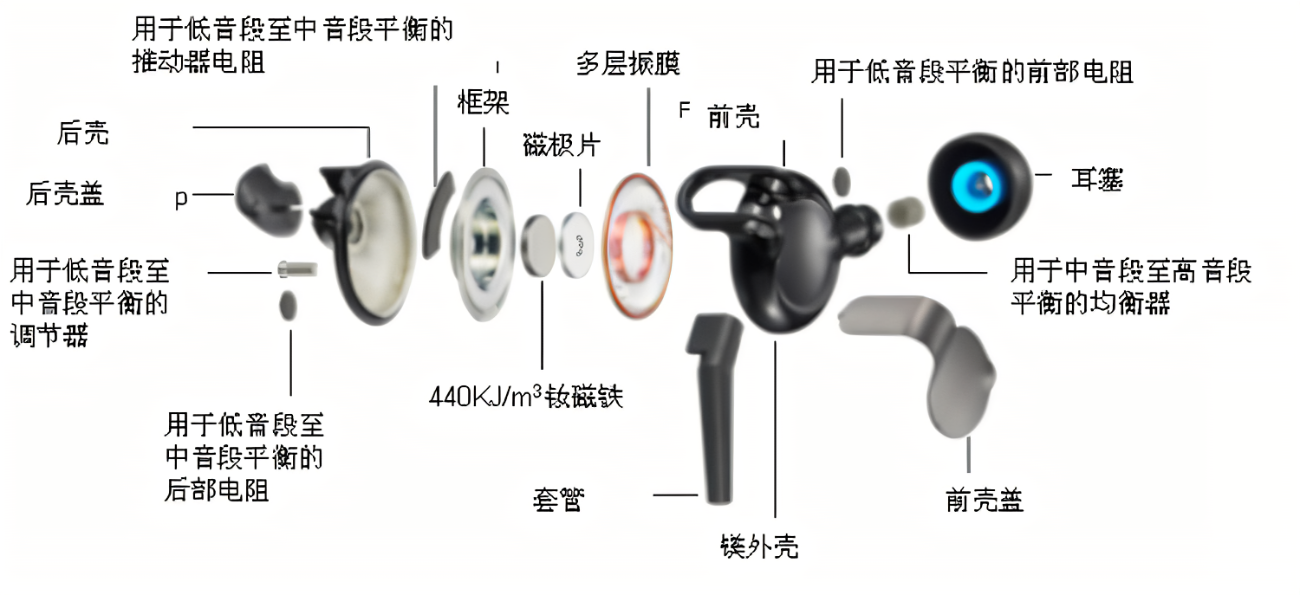
\includegraphics[width=0.6\textwidth]{dynamic_speaker.png}  % 建议替换为动圈扬声器原理示意图
    \caption{动圈式扬声器工作原理示意}
    \label{fig:dynamic_principle}
\end{figure}

\subsection{蓝牙特有:无线连接原理}
蓝牙耳机与音频源(如手机)的连接,需通过「蓝牙协议」完成信号传输,核心步骤如下,且全程工作在2.4GHz无线频段(与WiFi部分频段重叠,但通过跳频技术避免干扰):

\begin{enumerate}[label={\arabic*.}, itemsep=6pt]
    \item \textbf{配对:建立初始连接}  
          首次使用时,耳机长按「配对键」进入「配对模式」(指示灯闪烁),手机开启蓝牙后搜索耳机名称(如「XX-BT01」),选择后输入默认PIN码(多为0000或1234,现代机型多自动配对),完成连接后保存设备信息,后续靠近时自动连接。
    \item \textbf{编码:压缩音频信号}  
          手机将原始音频信号(如MP3、FLAC格式)通过蓝牙协议编码压缩:基础协议SBC(压缩率高、兼容性强,但音质损失略大),高端协议AAC(苹果设备主流,音质更优)、aptX(安卓设备常用,延迟低至40ms,适合游戏/通话)。
    \item \textbf{传输与解码:还原电信号}  
          编码后的信号以无线电波形式传输到耳机,耳机蓝牙模块接收后解码,将压缩信号还原为原始电信号,再传输至扬声器单元,最终完成声音播放。
\end{enumerate}
\clearpage

% 第四章:耳机的使用与维护指南(补充具体操作细节,增强实用性)
\section{耳机的使用与维护指南}
合理使用可延长耳机寿命(有线耳机寿命通常2-5年,蓝牙耳机电池寿命约2-3年),具体注意事项如下:

\begin{enumerate}[label={\arabic*.}, itemsep=6pt]
    \item \textbf{保护听力:控制音量与时长}  
          避免音量超过最大音量的60%(WHO建议安全音量),连续使用不超过1小时,中途休息5-10分钟;嘈杂环境(如地铁)尽量使用主动降噪耳机,避免为盖过噪音而调大音量。
    \item \textbf{清洁保养:定期清理污垢}  
          耳罩(皮质)用干布蘸少量酒精擦拭,避免水洗;入耳式耳塞(硅胶材质)可取下用肥皂水清洗,晾干后再安装;避免耳机接触汗液(运动后及时擦拭,防止腐蚀金属部件)。
    \item \textbf{存放与收纳:避免物理损伤}  
          有线耳机收纳时用「绕线器」整理线缆,避免用力拉扯或缠绕(防止内部导线断裂);头戴式耳机存放时避免挤压耳罩(防止海绵变形);蓝牙耳机长期不用时,需充电至50%后存放(避免电池过放损坏)。
    \item \textbf{蓝牙维护:优化连接与续航}  
          蓝牙耳机与设备距离不超过10米(蓝牙有效距离),避免遮挡(如金属壳手机可能削弱信号);电量低于20%时及时充电,避免长期耗尽电量(影响电池循环寿命);定期更新耳机固件(通过品牌APP),优化连接稳定性。
    \item \textbf{遵循规范:参考厂家指南}  
          不同品牌耳机(如索尼、森海塞尔)的维护细节可能不同,建议留存厂家提供的《使用说明书》,涉及维修(如电池更换)时选择官方售后,避免自行拆解损坏部件。
\end{enumerate}

% 第五章:结论(补充技术趋势,增强文档深度)
\section{结论}
耳机技术的发展围绕「音质提升」「体验优化」两大方向:从扬声器单元看,动圈式仍为主流,但动铁单元向多单元集成(如3单元、5单元)发展,静电单元逐步下放至中端机型;从连接方式看,蓝牙5.3及后续协议(如LE Audio)将进一步降低延迟(<20ms)、提升续航(较蓝牙5.0节能30%),并支持多设备同时连接(如耳机同时连手机和电脑)。

本文通过分类、结构、原理、维护的系统解析,明确了「通用耳机」与「蓝牙耳机」的技术差异,帮助读者跳出「所有耳机结构一致」的认知误区。若需深入了解蓝牙耳机芯片技术、主动降噪原理等细节,可参考专业电子技术平台文章:\href{https://www.elecfans.com/d/1109530.html}{《蓝牙耳机技术详解:从芯片到降噪》}(链接来自电子发烧友网,内容经行业工程师审核)。

\end{document}